\section{Enumeration}

Auch die zuvor besprochenen Regeln müssen ausgeführt und angewendet werden. Wie auch bei Pyro(J) wurde ein Button-up-Ansatz gewählt. Bei diesem Verfahren wird sich von unten nach oben durch den Baum gearbeitet. Erst wenn alle Regeln auf alle Sub-Bäume angewendet wurden, können die Regeln auch auf den Baum selbst angewendet werden. Die Komponente, die für das Ausführen und die Reihenfolge der Anwendung der Regel verantwortlich ist, ist der Enumerator. Für die hier vorgestellte Implementierung wurde ein Enumerator implementiert.


\subsection{Implementierung des Enumerators}

Bevor der Enumerator gestartet werden kann, muss er mit einer Regelmenge initialisiert werden. Die Regelmenge muss dabei dem Interface \texttt{RuleSet} entsprechen. Gestartet wird der Enumerator durch die Methode \texttt{apply(EquivalenceClass \&)}. Der Methode muss eine bisher noch nicht expandierte Äquivalenzklasse übergeben werden. 

Für jeden Planknoten der initialen Äquivalenzklasse wird die linke und rechte Äquivalenzklasse betrachtet. Wenn beide Klassen vorhanden sind, wird die Methode \texttt{apply(EquivalenceClass \&)} für die vorhandenen Äquivalenzknoten ausgeführt werden. Somit wird sichergestellt, dass die Regeln zuerst auf die untergeordneten Planknoten ausgeführt werden. Sobald die untergeordneten Pläne expandiert sind, wird die Regel ausgeführt. Da jede Regel neue Planknoten und neue Äquivalenzklassen hervorbringen kann, wird geprüft, ob bereits Äquivalenzklassen bekannt sind, die die selben Relationen repräsentieren. Lassen sich solche Knoten finden, werden die bereits bekannten statt der neu generierten Äquivalenzklassen verwendet. Falls ein tatsächlich unbekannter Knoten erzeugt wurde, wird zuerst auf diese Äuqivalenzklasse die Methode \texttt{apply} angewendet und diese Äuqivalenzklasse als bekannt gespeichert. Mit Hilfe dieser Methode wird verhindert, dass Berechnungen für Äquivalenzklassen mehrfach durchgeführt werden müssen. Die genaue Funktionalität kann mit Hilfe des Pseudocodes \ref{Pseudocode:enumerator} nachvollzogen werden.

\begin{figure}[ht]
  \centering
  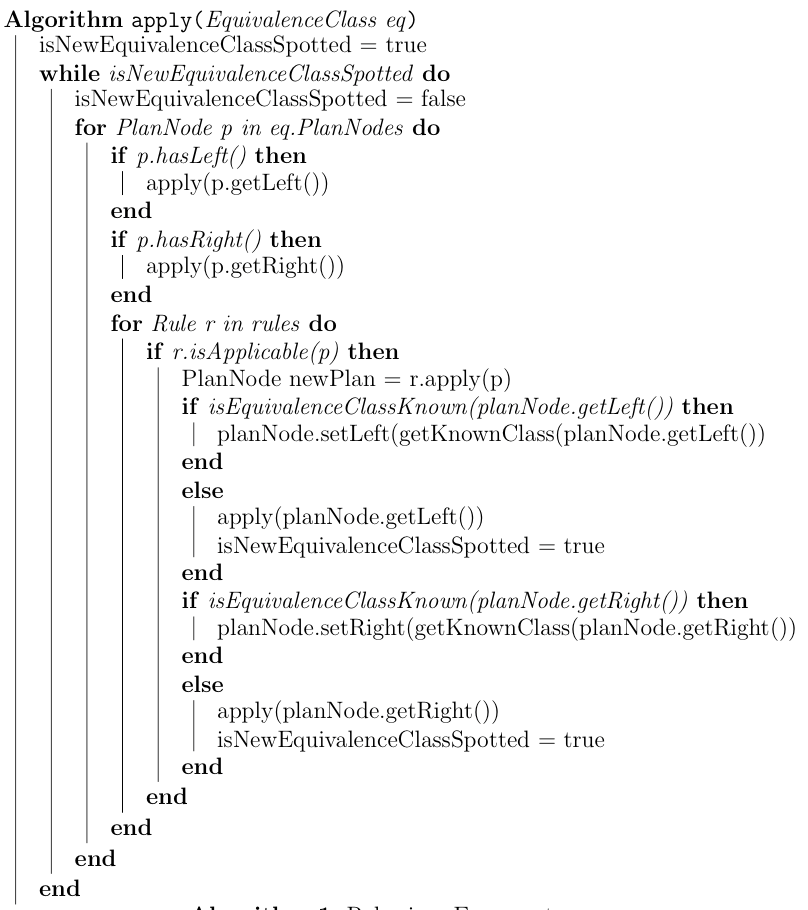
\includegraphics[scale=0.4]{04_Implementierung/00_media/Enumerator.png}
  \caption{Pseudocode: Rekursiver Enumerator (Enumerator 1)}
  \label{Pseudocode:enumerator}
\end{figure}



Neben diesem Enumerator (Enumerator 1) wurde auch der Enumeratoraus Pyro(J) (vgl. Abb. \ref{ExpandDAG}) implementiert. Im Gegensatz zu dem zuerst implementierten Enumerator, werden nicht alle Pläne erreicht. Insbesondere fällt auf, dass bei der Exchange Rule die neugebildeten Äquivaelnzklassen nicht mehr berücksichtige werden und die Regeln nicht mehr auf diese angewendet werden. Dies wird auch als möglicher Grund für die in Kapitel 3 gemessen Unvollständigkeit in Kapitel 5 beleuchtet.



\subsection{Erweiterbarkeit des Enumerators}

Schon das Interface des Emumerators ist erweiterbar. Andere Regelmengen können übergeben werden und so zur Ausführung kommen. Auch mit Hilfe des Template Parameters \texttt{PlanNode\_t} können die Planklassen ausgetauscht werden. Durch die Modularität der anderen Komponenten kann auch leicht ein neuer Enumerator implementiert werden, der den bisherigen ersetzt. Es muss kein spezielles Interface eingehalten werden. Daher muss bei der Erstellung eines neuen Enumerators nur die Exekutor Klasse verändert werden in der der bestehende Enumerator aufgerufen wird.